\documentclass[a4paper,twoside,BCOR=20mm]{scrreprt}
\usepackage[utf8]{inputenc}
\usepackage[T1]{fontenc}
\usepackage[ngerman]{babel}	% german hyphenation, quotes, etc
\usepackage[ngerman]{translator}
\usepackage{paralist}
\usepackage{amsfonts}
\usepackage{acronym}
\usepackage{enumerate}
\usepackage{hyperref}
\usepackage{amssymb}
\usepackage{caption}
\usepackage{multirow}
\usepackage{graphicx}
\usepackage{tabularx}
\usepackage{color}
\usepackage{wrapfig} % wrap text around figures
\usepackage{subfig} % align two pics beside each other
\usepackage[table,xcdraw]{xcolor}
\usepackage{enumitem} % für custom enumerations
\usepackage{float} % for better graphics placement
\usepackage{svg} % for scalable vector-graphics (see inkscape)
\setsvg{inkscapeexe=inkscape, inkscapeopt=-z -D} % set inkscape options
\svgpath{images/} % use dir 'images/' to search for svg files

\renewcaptionname{ngerman}{\figurename}{Abb.} % replace "Abbildung" with "Abb." for all captions for graphics

\hypersetup{ 					% ‘texdoc hyperref‘ for options
	pdftitle={PSE TECO: Pflichtenheft},
	pdfauthor={Jean Baumgarten, Oliver Liu, Patrick Ries, Erik Wessel, Thomas Frank},
	bookmarks=true,
}
\title{Pflichtenheft: PaVoS}

%Paket laden
\usepackage[
numberedsection,
nonumberlist, %keine Seitenzahlen anzeigen
acronym,      %ein Abkürzungsverzeichnis erstellen
toc,          %Einträge im Inhaltsverzeichnis
section]      %im Inhaltsverzeichnis auf section-Ebene erscheinen
{glossaries}

% KIT layout

\definecolor{orange}{rgb}{1,0.5,0}
\definecolor{mintgreen}{RGB}{50,161,137}
\definecolor{gray}{RGB}{120,120,120}

\usepackage[color]{changebar}
\cbcolor{gray}
\changebarwidth 0.5pt

\usepackage{fancyhdr}
\pagestyle{fancy}
 \fancyhf{} %alle Kopf- und Fußzeilenfelder bereinigen 
 
 \fancypagestyle{plain}{} %Kopf- und Fußzeile auf jeder Seite	 
	\fancyhead[L]{Pflichtenheft}
	\fancyhead[R]{\leftmark}
	\rhead{\nouppercase{\leftmark}}
	\renewcommand{\headrulewidth}{0.5pt}
	\renewcommand{\headrule}{\hbox to\headwidth{%
		\color{mintgreen}\leaders\hrule height \headrulewidth\hfill}}

\raggedbottom

	\renewcommand{\footrulewidth}{0.5pt}
	\renewcommand{\footrule}{\hbox to\headwidth{%
  		\color{mintgreen}\leaders\hrule height \headrulewidth\hfill}}				
	\fancyfoot[LE,RO]{\thepage}

\setcounter{tocdepth}{5}
\makeglossaries
\begin{document}
	
	\begin{titlepage}
	\begin{center}
	
\includegraphics[width=0.5\linewidth]{images/TECOLogo.png}\\[0.2cm]

	\textbf{TECO Research Group}\\[0.2cm]
	Marcel Köpke\\Matthias Budde\\Till Riedel\\
	\vspace{1cm}
	
	
\includegraphics[width=0.33\linewidth]{images/PaVoSLogo-Erweitert}\\[1cm]
	
	\textsc{\textbf{\LARGE Pflichtenheft}}\\
	{\small Version 0.1}\\
	
	\vspace{1cm}\hrule\vspace{0.4cm}
	\textbf{\huge Visualizing \& Mining of Geospatial Sensorstreams with Apache Kafka}\\
	\vspace{0.4cm}\hrule\vspace{1cm}
	
	{\Large Jean Baumgarten\\
	Oliver Liu\\
	Patrick Ries\\
	Erik Wessel\\
	Thomas Frank\\}

	\vspace{1cm}
	\today
	
	\end{center}
\end{titlepage}
	\tableofcontents
	\chapter{Zielbestimmung}
Das Produkt dient der Verarbeitung und Darstellung von Sensordatenstreams. Durch die übersichtliche Visualisierung der Daten auf einer Karte wird die schnelle Analyse von großen Datenmengen ermöglicht und der Zeitaufwand wird minimiert.\\
Ein Hauptmerkmal unseres Produktes ist die Fähigkeit, zusätzlich zu Echtzeitdaten auch historische Datenbestände zu verarbeiten und zu exportieren.
\section{Musskriterien}
\subsection{Backend (Server)}
\begin{enumerate}[label=\textbf{MK\arabic{enumi}0}]
	\setcounter{enumi}{99}
	\item Der Server kann Sensordaten empfangen
	\item Eingeführte Sensordaten werden gesichert
	\item Neue Sensordaten werden zeitnah an alle Instanzen des Webinterfaces weitergeleitet und dargestellt
	\item Der Dienst ist logisch modular aufgebaut und erlaubt das Ergänzen und Ersetzen von einzelnen funktionalen Modulen, wie z.B. verschiedene Exportformate, Zwischenmodule
	\item Der Server verarbeitet und speichert Daten für spätere Verwendung
	\item Der Server kann vorverarbeitete und gespeicherte Daten abrufen
	\item Der Server unterstützt skalar- und vektorwertige Sensortypen
\end{enumerate}
\subsection{Frontend (Webinterface)}
\begin{enumerate}[label=\textbf{MK\arabic{enumi}0}]
	\setcounter{enumi}{199}
	\item Das Webinterface unterstützt die rasterisierte Darstellung der Sensordaten auf einer Weltkarte in Form von vordefinierten Shapes
	\item Das Webinterface unterstützt die Darstellung einer auf Deutschland beschränkten Ansicht
	\item Der Nutzer kann aktuelle und historische Sensordaten über das Webinterface darstellen lassen
	\item Der Nutzer kann die Sensordaten über das Webinterface herunterladen
	\item Der Nutzer kann kürzlich beobachtete Daten als Wiederholung anzeigen lassen
	\item Das Webinterface unterstützt die Darstellung von erweiterten Informationen bzgl. der Sensordaten in Form von Graphen
	\item Die Standardsprache des Webinterfaces ist Englisch
	\item Das Webinterface kann parallel von mehreren Nutzern aufgerufen und benutzt werden
\end{enumerate}

\section{Wunschkriterien}
\subsection{Backend (Server)}
\begin{enumerate}[label=\textbf{WK\arabic{enumi}0}]
	\setcounter{enumi}{99}
	\item Der Server skaliert mit unterschiedlich großen Datenmengen
	\item Der Server läuft auch mit fehlerhaften Daten stabil
	\item Der Server überarbeitet im Leerlauf fehlerhafte Daten aus der Datenbank
	\item Der Server unterstützt das Hinzufügen von neuen Anzeigesprachen für das Webinterface
	\item Der Server unterstützt den Import von historischen Daten im NetCDF-Format und kann diese Daten problemlos verarbeiten
	\item Der Server unterstützt das Filtern von ausgegebenen und angezeigten Daten
	\item Der Server kann durch eine Admin-GUI gesteuert werden
	\item Der Server gibt aussagekräftige Fehlermeldungen aus
\end{enumerate}
\subsection{Frontend (Webinterface)}
\begin{enumerate}[label=\textbf{WK\arabic{enumi}0}]
	\setcounter{enumi}{199}
	% Zoom / Darstellung
	\item Der Nutzer kann die Karte in vordefinierten Detaillierungsgraden darstellen lassen
	\item Die Genauigkeit der Darstellung von Clustern wird entsprechend der Zoom-Stufe angepasst
	\item Die Approximation von Clustern führt nicht zu größeren Diskrepanzen oder Wartezeiten
	\item Die Erzeugung der grafischen Komponenten erfolgt zeitnah und parallel zur Darstellung der Benutzeroberfläche selbst
	\item Der Nutzer kann verschiedene Sensordatentypen (Feinstaub, Wind, Temperatur, etc.) an- bzw. ausschalten
	% Favoriten
	\item Der Nutzer kann Standorte als Favoriten abspeichern
	\item Der Nutzer kann Gebiete als Kombination von Clustern auswählen und diese als Favoriten abspeichern
	\item Der Nutzer kann favorisierte Standorte/Gebiete auswählen um schnell und einfach die optimale Ansicht des gewählten Standortes/Gebiets dargestellt zu bekommen
	\item Der Nutzer kann favorisierte Standorte/Gebiete in einer grafischen Darstellung vergleichen, z.B. nebeneinander als Split-Panel
	\item Der Nutzer kann zwischen mehreren Ansichten wechseln, um die Standardansicht oder geladene Szenarien darzustellen
	\item Der Nutzer kann einzelne Sensoren/Cluster aus der Darstellung ausschließen
	\item Der Nutzer kann Anzeigefilter einstellen
	\item Der Nutzer kann Anzeigefilter als Favoriten speichern
	% Fehler bei Sensoren
	\item Der Nutzer kann fehleranfällige Sensoren melden
	\item Dem Nutzer wird eine Warnung angezeigt, wenn das Abrufen von Sensordaten nicht möglich ist
	\item Bei fehlenden Sensordaten kann ein Standardwert oder ein approximierter Wert anhand von Umgebungsinformationen ermittelt und angezeigt werden
	% Aktualisierung
	\item Der Nutzer kann zwischen einer automatischen und einer manuellen Aktualisierung von Echtzeitsensordaten wechseln
	\item Der Nutzer kann die Aktualisierungsrate von Echtzeitdaten einstellen
	% Laden
	\item Der Nutzer kann Sensordaten in vielen gebräuchlichen Formaten herunterladen
	% Benachrichtigungen
	\item Der Nutzer kann Benachrichtigungen mit Bedingungen einstellen, die dem Nutzer die aktuellen Daten melden, falls die Bedingungen erfüllt sind
	\item Auf Graphen werden Bedingungen für Benachrichtigungen als Grenzwerte angezeigt
	\item Der Nutzer kann Töne und Farben für Benachrichtigungen festlegen
	% Sonstiges
	\item Für standardisierte Displayauflösungen wird immer eine benutzerfreundliche Darstellung angeboten
	\item Der Nutzer kann eine Anzeigesprache auswählen
	\item Die Anwendung speichert automatisch die Einstellungen und Favoriten des Nutzers über Browsersessions hinweg (Cookies)
\end{enumerate}

\section{Abgrenzungskriterien}
\begin{enumerate}[label=\textbf{AK\arabic{enumi}0}]
	\setcounter{enumi}{99}
	\item Der Server speichert Sensordaten nicht auf unbegrenzte Zeit und in unbegrenzter Menge
	\item Der Server speichert keine Daten von Nutzern und deren Aktivitäten/Interaktionen mit dem Webinterface
	\item Der Datendurchsatz des Servers wird durch lokale Netzwerkgeschwindigkeiten beschränkt
	\item Der Server ist nicht in der Lage, korrekte Vorhersagen zu erstellen
	\item Der Server ist nicht in der Lage, Sensordaten von fehlerhaften Sensoren auszuwerten
	\item Der Server ist nicht in der Lage, unbegrenzt viele Daten anzuzeigen und zu aktualisieren
	\item Der Server ist nicht in der Lage, durch Störungseinflüsse veränderte Sensordaten zu erkennen
	\item Der Server unterstützt keine weiteren Eingabeformate als Apache Kafka Streams (und, falls \textbf{WK1070} erfüllt ist, NetCDF-Dateien)
	\item Der Server unterstützt nicht das manuelle Hinzufügen von neuen Sensordaten
\end{enumerate}
	\chapter{Produkteinsatz}
Das Produkt ermöglicht es seinen Nutzern, Echtzeitdaten sowie archivierte Daten vieler Sensoren von unterschiedlichen Messgrößen abzurufen und darzustellen. Es bietet dem Nutzer hierfür eine moderne und intuitive webbasierte Bedienoberfläche. Weiterhin ermöglicht das Produkt dem Nutzer über eine öffentliche Schnittstelle den direkten Zugriff auf die Daten. Unter anderem können diese Daten als Archivdatei exportiert werden. Durch die modulare Architektur unseres Produkts werden vielseitige Einsatzmöglichkeiten außerhalb der Luftqualitätsmessung ermöglicht.
\section{Anwendungsbereiche}
\begin{itemize}
	\item Analyse und Visualisierung von Sensordaten
	\item Archivierung von Sensordaten
\end{itemize}
\section{Zielgruppe}
\begin{itemize}
	\item Personen, die Sensordaten auswerten und visuell darstellen wollen. Dazu gehören:
	\begin{itemize}
		\item Wissenschaftler
		\item Privatpersonen, die mit Sensoren arbeiten
	\end{itemize}
	\item Personen, die Sensordaten sammeln und archivieren wollen
	\item generelle Bevölkerung, um Informationen über aktuelle Werte von Sensoren zu erhalten, z.B. über Luftverschmutzung, Temperatur usw.
\end{itemize}

	\chapter{Produktumgebung}
Das Produkt läuft mit Client-Server Architektur im "Thin Client" Konzept.
\section{Software}
\subsection{Server}
\begin{itemize}
	\item Linux-Betriebssystem (min. Debian 8)
	\item Java-Anwendung mit Java 8
	\item Java Web-Dienst mit Eclipse Jetty
	\item Datenbank mit PostgreSQL
\end{itemize}
\subsection{Client}
\begin{itemize}
	\item Webbrowser, Referenzstandard Mozilla Firefox 57
\end{itemize}
\section{Hardware}
\subsection{Server}
\begin{itemize}
	\item Aus dem Internet erreichbarer, leistungsstarker Rechner
\end{itemize}
\subsection{Client}
\begin{itemize}
	\item Standardrechner mit genügend Leistung für Firefox (min. 512MB RAM, 512MB Festplattenspeicher, 1.5GHz CPU)
\end{itemize}
	\chapter{Funktionale Anforderungen}
\begin{enumerate}[label=\textbf{PF\arabic{enumi}0}]
	\setcounter{enumi}{99}
	\section{Pflicht Funktionale Anforderungen}
	\subsection{Server}

	\item \textbf{Englisch als Systemsprache}\\
		Das System wird nur die Englische Sprache unterstützen und alles in Englisch anzeigen. 
	
	\item \textbf{Sensordaten empfangen} \label{A1}\\
		Beim ersten öffnen der Server Admin GUI soll sich der Nutzer aufgefordert werden einen Kafka Daten stream mit Sensordaten einzufügen oder komprimierte Sensordaten zu importieren. Beim Einfügen oder importieren wird von dem Programm überprüft ob es sich für das Programm lesbare Formate handelt, wenn nicht gibt das Programm eine Fehlermeldung aus und schreibt den Grund in eine Logdatei.  
		
	\item \textbf{Sensordaten werden gesichert}\\
		Die Sensordaten werden extrahiert und in mehre Streams aufgeteilt und gruppiert und in einem Datenerhaltungssystem gespeichert. Falls es bei diesem Prozess zu Fehlern kommt, wie dass die Gruppierung fehlschlägt oder kein gültiges Datenerhaltungssystem verfügbar ist, wird auch eine Fehlermeldung ausgegeben und in eine Logdatei geschrieben.
		
	\item \textbf{Verarbeitung der Daten für Kartenansicht} \label{FAKarten}\\
		Der Dienst verarbeitet so vor, dass sie für spätere Verwendungen genutzt werden wie die Weiterleitung an den Webinterface und auf einer gerasterten Karte angezeigt werden können.
	
	\item \textbf{Verarbeitung der Daten für Mittelwertberechnung} \label{FAMittel}\\
		Der Dienst verarbeitet die Daten so vor, dass Mittelwerte berechnet werden von den Sensordaten um diese zur Analyse weiter an das Web-Interface zu geben.
	
	\item \textbf{Verarbeitung der Daten für Export}\\
		Der Dienst verarbeitet die Daten so vor, dass sie komprimiert exportiert werden können aus dem dem Datenerhaltungssystem damit diese im Web-Interface downloadet werden können.
	
	\item \textbf{Kann gespeicherte Daten wieder abfragen}\\
		Der Dienst kann die vorbearbeiteten Daten  \ref{FAKarten},\ref{FAMittel} jeder Zeit wieder aufrufen und weiterleiten an das Webinterface.
		
	\item \textbf{Daten werden an Webinterface gesendet} \label{FAWebsend}\\
		Die Daten aus dem Datenerhaltungssystem und vom Kafka Stream können an das Webinterface gesendet werden.
	 	
	 \item \textbf{Hinzufügen weiter Module}\\
		 Der Dienst ist so aufgebraucht, dass es dem Nutzer und Programmierer möglich sein wird, auf dem einzelnen Interface zuzugreifen und so neue Module für den Dienst zu entwickeln um das System zu erweitern. Ein Beispiel wäre neue Exportformate hinzuzufügen oder ein Modul zwischen Server-Dienst und Webinterfaces zu setzten. 
	 
	 \item \textbf{Der Dienst unterstützt skalar- und vektorwertige Sensortypen}
	 	Der Dienst unterstützt beim Kafka Stream und beim Import von Sensor Daten nur Skalar Sensortypen und vekorwertige Sensortypen. Falls andere Sensortypen im Stream entdeckt werden, dann wird dem Nutzer eine Anleitung angezeigt wie er selbst ein neuen Sensortyp hinzufügen kann.
 
	 \subsection{Webinterface}

	 \item \textbf{Sensordaten werden dargestellt}\\
	 	Nach dem die Sensordaten \ref{FAWebsend} empfangen wurden auf dem Webinterface können sie auf dem Webinterface dargestellt werden
	 
	 \item \textbf{Darstellung der Daten}\\
	 	Auf dem Webinterface kann man die Sensordaten in verschiedenen Rastern (Beispiel: Quadratenraster) auf einer Weltkarte darstellen mit vordefinierten Formen wie zum Beispiel: Quadrate oder Hexagone.
	 
	 \item \textbf{Darstellung nur auf Deutschland}\\
	 	Auf dem Webinterface kann man das Land Deutschland anzeigen lassen und sonst keine anderen Länder. So ist die Ansicht nur auf Deutschland beschränkt.
	 
	 \item \textbf{Sensordaten anzeigen}\\
		Auf dem Webinterface kann man aktuellsten Daten von Sensoren anzeigen lassen auf der Karte und auch ältere Daten von Sensoren anzeigen lassen auf der Karte.
		
	\item \textbf{Export von Daten}\\
		Auf dem Webinterface kann man die aktuellen Daten und die historischen Daten exportieren in einem vordefinierten Format in Form einem Download. 
		
	\item \textbf{Wiederholung anzeigen}\\
		Auf dem Webinterface kann man aktuelle und historische Daten mit Hilfe von einem Slider als Wiederholung anzeigen lassen.
		
	\item \textbf{Mehrere Instanzen des Webinterface}\\
		Mehre Instanzen des Webinterfaces werden aufrufbar sein, so dass mehre Nutzer gleichzeitig mit den Sensordaten arbeiten können.
		
	\item \textbf{Detail Ansicht von Sensoren}\\
		Auf dem Webinterface kann man von einzelnen Sensoren eine Detailansicht darstellen um so nähere Informationen über den Sensor zu erhalten. Es wird dann auch eine Möglichkeit geben genauere Statistiken von dem Sensor in Form von Graphen und Text anzuzeigen.
\end{enumerate}

\begin{enumerate}[label=\textbf{WF\arabic{enumi}0}]
	\setcounter{enumi}{99}
	\section{Wunsch Funktionale Anforderungen}
	
	\subsection{Server}
	
	\item \textbf{Der Dienst sucht nach Fehlerhaften Sensordateien}\\
	Der Dienst überprüft im Datenerhaltungssystem ob Sensordaten Outlier sein können und gibt den Nutzer eine Meldung, was an den Daten ungewöhnlich ist und ihm die Möglichkeit diese zu löschen.
	 
	\item \textbf{Mehrere Sprachen}\\
	Der Dienst kann mit mehren Sprachen außer Englisch umgehen und die Anzeigesprache kann auch entsprechen geändert werden. 
	
	\item \textbf{Fitern von Daten}\\
	Man kann auf der Admin GUI die Daten oder Streams filtern, damit nur bestimmte Daten weiter verarbeitet werden.
	
		
	\subsection{Webinterface}
\end{enumerate}
	
	 
	  

	\chapter{Produktdaten}
\section{Server}
\begin{enumerate}[label=\textbf{PD\arabic{enumi}0}]
	\setcounter{enumi}{99}
	\item \textbf{Sensordaten}\\
	Sowohl vorverarbeitete Sensordaten als auch Echtzeitsensordaten werden vom Server bis zu einer gewissen Menge gespeichert.
\end{enumerate}
\section{Webinterface}
\begin{enumerate}[label=\textbf{PD\arabic{enumi}0}]
	\setcounter{enumi}{199}
	\item \textbf{Cookies}\\
	Die vom Nutzer gesetzten Einstellungen (z.B. Zoom-Stufe, an- bzw. ausgeschaltete Sensordatentypen), Favoriten (z.B. Gebiete, Anzeigefilter) und Benachrichtigungen werden in Form von Cookies im Browser des Nutzers gespeichert.
\end{enumerate}
	\chapter{Nichtfunktionale Anforderungen}
\begin{enumerate}[label=\textbf{NF\arabic{enumi}0}]
	\setcounter{enumi}{99}
	
	\item \textbf{Anzeigesprache}\\
	Die Standardanzeigesprache des Webinterfaces ist Englisch.
	
	\item \textbf{Parallele Zugriffe}\\
	Das Webinterface muss von bis zu 100 Nutzern gleichzeitig bedient werden können. Alle folgenden Anforderungen gelten nur für bis zu 100 parallele Nutzer. Für mehr Nutzer sind keine Leistungsgarantien gegeben.
	
	\item \textbf{Sichtbare Cluster}\\
	Das Webinterface muss bis zu 1000 Cluster gleichzeitig anzeigen können. Alle folgenden Anforderungen gelten nur für bis zu 1000 sichtbare Cluster. Für mehr Cluster sind keine Leistungsgarantien gegeben.
	
	\item \textbf{Zoomstufen}\\
	Das Webinterface muss je nach Ansicht 4 bis 5 unterschiedliche Zoomstufen unterstützen.
	
	\item \textbf{Verzögerung von neuen Daten}\\
	Neue Echtzeitsensordaten werden innerhalb einer Minute verarbeitet und auf allen Instanzen der Webinterface angezeigt.
	
	\item \textbf{Verzögerung von historischen und archivierten Daten}\\
	Historische und archivierte Daten, die eine große Datenmenge umfassen und/oder von einem persistenten Speicher geladen werden müssen, benötigen mehr Zeit zur Verarbeitung und Visualisierung. Für diese sind keine Leistungsgarantien gegeben.
	
	\item \textbf{Speicherung von kürzlichen Echtzeitsensordaten}\\
	Kürzliche Echtzeitsensordaten werden bis zu einer Gesamtgröße von 1GB in dem Arbeitsspeicher gespeichert. Diese kürzlichen Daten können schneller abgerufen werden als ältere Daten und werden für die Wiederholungsansicht verwendet.
	
	\item \textbf{Speicherung von älteren Echtzeitsensordaten}\\
	Alle an Apache Kafka angelegte Sensordaten werden von Apache Kafka in einem persistenten Speicher gespeichert. Die Größe des Speichers begrenzt die Menge der gespeicherten Daten.
	
	\item \textbf{Skalierbarkeit}\\
	Der Server startet automatisch neue Worker-Container um Sensordaten und Anfragen des Servers zu verarbeiten. Mindestens 10 Worker können je nach Bedarf gestartet und beendet werden.
	
	\item \textbf{Stabilität}\\  
	Der Server muss im normalen Betrieb problemlos mit unerwarteter Terminierung von einem oder mehreren Worker-Containern umgehen und innerhalb von fünf Minuten die ursprüngliche Rechenleistung wiederherstellen. Fehler in den Eingabedaten wie ungültige Werte oder Syntaxfehler führen nicht zu einem Absturz des Servers.
	
	\item \textbf{Reaktionszeit}\\
	Das Webinterface muss innerhalb von zwei Sekunden auf Interaktionen des Nutzers reagieren. Falls der Webserver bis dahin nicht das erwünschte Ergebnis liefern kann, wird der Nutzer darauf hingewiesen.
	
	\item \textbf{Ladezeiten der Darstellungselemente}\\
	Ein Zugriff auf das Webinterface lädt Darstellungselemente wie Cluster-Shapes, Graphen und Buttons innerhalb von 5 Sekunden.
	
	\item \textbf{Genauigkeit der Clusterberechnung}\\
	Die Approximation der Daten in Clustern darf nicht zu einer Abweichung über 5\% von Ergebnissen einer akkuraten Berechnung führen.
	
	\item \textbf{Geschwindigkeit der Clusterberechnung}\\
	Die Approximation der Daten in Clustern darf nicht mehr als 2 Sekunden dauern.
	
	\item \textbf{Aktualisierungsgeschwindigkeit}\\
	Die Karte aktualisiert Echtzeitsensordaten alle 10 Sekunden.

\end{enumerate}
	
	\chapter{Qualitätssicherung}
	\label{ch:Qualitaetssicherung}
	
	Für die Komponententests unseres Systems verwenden wir grundsätzlich JUnit. Für weiterführenden Tests werden im folgenden Abschnitt Szenarien beschrieben.
	
\section{Globale Testszenarien}
	\label{ch:Qualitaetssicherung:sec:GlobaleTestszenarien}
	
\subsection{Server}
\begin{enumerate}[label=\textbf{TI\arabic{enumi}0}]
	\setcounter{enumi}{99}
	
	\item \textbf{Erstanwendung der Konfigurations-GUI mit Kafka Stream}\\
		Die Konfigurations-GUI wurde noch nie gestartet und es steht ein Kafka Stream namens 'TestStream' bereit.\\
		Der Nutzer startet die Konfigurations-GUI, woraufhin diese ihn auffordert, den hinzuzufügenden Kafka Stream auszuwählen.\par
		
		Der Nutzer schreibt 'TestStream' in das Feld des Popups und bestätigt.\\
		Die Konfigurations-GUI akzeptiert den Stream und fügt ihn hinzu.
	\item \textbf{Erstanwendung der Konfigurations-GUI ohne Kafka Stream}\\
		Die Konfigurations-GUI wurde noch nie gestartet und es steht kein Kafka Stream bereit.\\
		Der Nutzer startet die Konfigurations-GUI, woraufhin diese ihn auffordert, den hinzuzufügenden Kafka Stream auszuwählen.\par
		
		Der Nutzer schreibt 'TestStream' in das Feld des Popups und bestätigt.\\
		Die Konfigurations-GUI akzeptiert den Stream nicht und fordert ihn erneut auf, den hinzuzufügenden Kafka Stream auszuwählen.
	\item \textbf{Hinzufügen von zusätzlichen Streams zur Konfigurations-GUI mit Kafka Stream}\\
		Die Konfigurations-GUI ist gestartet, es ist ein Kafka Stream namens 'TestStream' hinzugefügt worden und es steht ein Kafka Stream namens 'TestStream2' bereit.\\
		Der Nutzer wählt die Option 'Stream hinzufügen', woraufhin die Konfigurations-GUI ihn auffordert, den hinzuzufügenden Kafka Stream auszuwählen.\par
		
		Der Nutzer schreibt 'TestStream2' in das Feld des Popups und bestätigt.\\
		Die Konfigurations-GUI akzeptiert den Stream und fügt ihn hinzu.
	\item \textbf{Hinzufügen von zusätzlichen Streams zur Konfigurations-GUI ohne Kafka Stream}\\
		Die Konfigurations-GUI ist gestartet, es ist ein Kafka Stream namens 'TestStream' hinzugefügt worden und es steht kein Kafka Stream bereit.\\
		Der Nutzer wählt die Option 'Stream hinzufügen', woraufhin die Konfigurations-GUI ihn auffordert, den hinzuzufügenden Kafka Stream auszuwählen.\par
		
		Der Nutzer schreibt 'TestStream' in das Feld des Popups und bestätigt.\\
		Die Konfigurations-GUI akzeptiert den Stream nicht und fordert ihn erneut auf, den hinzuzufügenden Kafka Stream auszuwählen.
	\item \textbf{Entfernen von Streams in der Konfigurations-GUI}\\
		Die Konfigurations-GUI ist gestartet und es ist ein Kafka Stream namens 'TestStream' hinzugefügt worden.\\
		Der Nutzer wählt die Option 'Stream entfernen', woraufhin die Konfigurations-GUI ihn auffordert, den zu entfernenden Kafka Stream auszuwählen.\par
		
		Der Nutzer schreibt 'TestStream' in das Feld des Popups und bestätigt.\\
		Die Konfigurations-GUI entfernt den Stream.
	\item \textbf{Export einer Archiv-Datei in der Konfigurations-GUI}\\
		Die Konfigurations-GUI ist gestartet und es ist ein Kafka Stream namens 'TestStream' hinzugefügt worden.\\
		Der Nutzer wählt die Option 'Export Stream', woraufhin die Konfigurations-GUI ihn auffordert, den Dateityp, das Verzeichnis und den Namen der zu exportierenden Archiv-Datei auszuwählen.\par
		
		Der Nutzer wählt das Format
		\begin{itemize}
		\item NetCDF
		\item CSV
		\end{itemize}
		, wählt das Verzeichnis 'SensorExport' bzw. erstellt es, falls es noch nicht existiert, legt den Namen auf 'TestSensorExport' fest und bestätigt.\\
		Die Konfigurations-GUI exportiert den Stream.
	\item \textbf{Import einer Archiv-Datei in der Konfigurations-GUI}\\
		Die Konfigurations-GUI ist gestartet, es ist ein Kafka Stream namens 'TestStream' hinzugefügt worden und es existiert eine importierbare Archiv-Datei im Verzeichnis 'SensorExport' mit dem Namen 'TestSensorExport'.\\
		Der Nutzer wählt die Option 'Import Stream', woraufhin die Konfigurations-GUI ihn auffordert, die zu importierenden Archiv-Datei auszuwählen.\par
		
		Der Nutzer wählt die
		\begin{itemize}
		\item NetCDF
		\item CSV
		\end{itemize}
		Datei und bestätigt.\\
		Die Konfigurations-GUI importiert den Stream.
	\item \textbf{Clusterform in der Konfigurations-GUI festlegen}\\
		Die Konfigurations-GUI ist gestartet und es ist ein Kafka Stream namens 'TestStream' hinzugefügt worden.\\
		Der Nutzer wählt die Option 'Select Clusterform', woraufhin die Konfigurations-GUI ihn auffordert, aus mehreren Möglichkeiten eine Form für die Cluster zu berechnen.\par
		
		Der Nutzer wählt die
		\begin{itemize}
		\item Quadrat
		\item Hexagon
		\end{itemize}
		Form und bestätigt.\\
		Die Konfigurations-GUI akzeptiert die neue Clusterform und berechnet Mittelwerte und Clusterpositionen neu.
	\item \textbf{Clustergröße in der Konfigurations-GUI festlegen}\\
		Die Konfigurations-GUI ist gestartet und es ist ein Kafka Stream namens 'TestStream' hinzugefügt worden.\\
		Der Nutzer wählt die Option 'Change Clustersize', woraufhin die Konfigurations-GUI ihn auffordert, einen Wert innerhalb eines Bereiches einzutragen.\par
		
		Der Nutzer wählt die Größe '2' und bestätigt.\\
		Die Konfigurations-GUI akzeptiert die neue Clusterform und berechnet Mittelwerte und Clusterpositionen neu.

\end{enumerate}

\subsection{Webinterface}
\begin{enumerate}[label=\textbf{TI\arabic{enumi}0}]
	\setcounter{enumi}{199}
	
	\item \textbf{Darstellung des berechneten Mittelwertes im Webinterface}\\
		Das Webinterface ist gestartet und es ist ein Kafka Stream namens 'TestStream' hinzugefügt worden. Die Ansicht des Webinterfaces ist auf Karlsruhe in Deutschland fokussiert.\\
		Der Nutzer wählt alle Skalierungsstufen der Karte in sich entfernender Reihenfolge aus, woraufhin die berechneten Mittelwerte auf der Karte als Farbe der Cluster zu sehen sind.\par
	\item \textbf{Darstellung von Clustern ohne Sensoren im Webinterface}\\
		Das Webinterface ist gestartet und es ist ein Kafka Stream namens 'TestStream' hinzugefügt worden. Die Ansicht des Webinterfaces ist auf Karlsruhe in Deutschland fokussiert. Es existiert ein Cluster ohne Sensoren in seinem Einflussgebiet, hier auch 'leerer Cluster' genannt.\\
		Der Nutzer wählt alle Skalierungsstufen der Karte in sich entfernender Reihenfolge aus. Die Karte zeigt leere Cluster nicht an.\par
	\item \textbf{Darstellung der tabellarischen Ansicht im Webinterface}\\
		Das Webinterface ist gestartet, es ist ein Kafka Stream namens 'TestStream' hinzugefügt worden. Die Ansicht des Webinterfaces ist auf Karlsruhe in Deutschland fokussiert.\\
		Der Nutzer wählt in der Ansicht den tabellarischen Modus.\\
		Daraufhin stellt das Webinterface die Sensordaten in einer geordneten Tabelle dar.\par
		
		Der Nutzer selektiert dann den Parameter 'Name', woraufhin das Webinterface die Sensoren nach Namen alphabetisch sortiert.
	\item \textbf{Benutzung mehrerer Webinterface-Instanzen}\\
		Das Webinterface ist nicht geöffnet, es ist ein Kafka Stream namens 'TestStream' hinzugefügt worden und im Browser sind Daten des Webinterfaces gespeichert. Die Ansicht des Webinterfaces ist auf Karlsruhe in Deutschland fokussiert.\\
		Der Nutzer öffnet das Webinterface für jede mögliche Ansicht einmal mehr in unterschiedlichen Tabs oder Fenstern des Browsers.\\
		Das Webinterface lädt auf allen Instanzen zu Beginn die gleichen Ansichten.\par
		
		Anschließend wählt der Nutzer pro Instanz verschiedene Ansichten.\\
		Das Webinterface stellt pro Instanz eine Ansicht dar. Die Ansichten der Instanzen werden nach der Auswahl gleichzeitig angezeigt.
	\item \textbf{Auswahl eines Sensortyps im Webinterface}\\
		Das Webinterface ist geöffnet und es ist ein Kafka Stream namens 'TestStream' hinzugefügt worden. Die Ansicht des Webinterfaces ist auf Karlsruhe in Deutschland fokussiert.\\
		Der Nutzer wählt im Webinterface die darzustellenden Sensortypen aus. Er aktiviert nur den Sensortyp 'Feinstaub'.\\
		Das Webinterface stellt daraufhin nur noch die Werte für 'Feinstaub'-Sensoren dar.\par
	\item \textbf{Export einer Archiv-Datei aus dem Webinterface}\\
		Das Webinterface ist geöffnet und es ist ein Kafka Stream namens 'TestStream' hinzugefügt worden.\\
		Der Nutzer wählt die Option 'Export Sensordata' und wählt das Format 'NetCDF', woraufhin das Webinterface den browserspezifischen Download-Dialog öffnet.\\
		Der Nutzer wählt das Verzeichnis 'SensorExport' bzw. erstellt es, falls es noch nicht existiert, legt den Namen auf 'TestSensorExport' fest und bestätigt.\par
		
		Der Nutzer wählt das Format
		\begin{itemize}
		\item NetCDF
		\end{itemize}
		, wählt das Verzeichnis 'SensorExport' bzw. erstellt es, falls es noch nicht existiert, legt den Namen auf 'TestSensorExport' fest und bestätigt.\\
		Die Konfigurations-GUI exportiert den Stream.
	\item \textbf{Wiederholungen im Webinterface anzeigen}\\
		Das Webinterface ist geöffnet und es ist ein Kafka Stream namens 'TestStream' hinzugefügt worden.\\
		Der Nutzer wählt im Webinterface eine Zeit aus oder verschiebt den Zeitregler 1 Minute zurück. \\
		Das Webinterface stellt daraufhin eine Wiederholung der Sensordaten von der Ausgewählten Zeit bis zum aktuellen Zeitpunkt dar.\par
		
		Der Nutzer kann mit einem Klick auf den 'Pause' Knopf die Wiederholung anhalten. Drückt er anschließend wieder auf 'Play', läuft die Wiederholung weiter.
	\item \textbf{Echtzeitdarstellung im Webinterface}\\
		Das Webinterface ist geöffnet, es ist ein Kafka Stream namens 'TestStream' hinzugefügt worden und das Webinterface zeigt eine Wiederholung an.\\
		Der Nutzer wählt 'Live' aus, woraufhin das Webinterface wieder die Echtzeitdaten darstellt und den Zeitregler wieder zurück auf 'Live' stellt.\par
	\item \textbf{Detailansicht eines Sensors im Webinterface anzeigen}\\
		Das Webinterface ist geöffnet und es ist ein Kafka Stream namens 'TestStream' hinzugefügt worden.\\
		Der Nutzer wählt in der Ansicht einen Sensor aus.\\
		Das Webinterface stellt daraufhin eine detaillierte Auflistung der Sensoreigenschaften dar.\par
	\item \textbf{Melden eines Sensors im Webinterface}\\
		Das Webinterface ist geöffnet und es ist ein Kafka Stream namens 'TestStream' hinzugefügt worden.\\
		Der Nutzer wählt in der Ansicht einen Sensor aus und klickt auf die Schaltfläche 'Report Sensor'. Anschließend schreibt der Nutzer in das Feld 'Reason' den Grund des Meldens an. Hier ist dieser Grund 'TestReportReason'.\\
		Das Webinterface zeigt dem Nutzer daraufhin an, dass die Meldung des Sensors erfolgt ist und speichert sie ab.\par
		
\end{enumerate}
	\chapter{Systemmodelle}

\section{Anwendungsfälle}
    % Anwendungsfall Webinterface
    \subsection{Bedienung des Webinterface}
        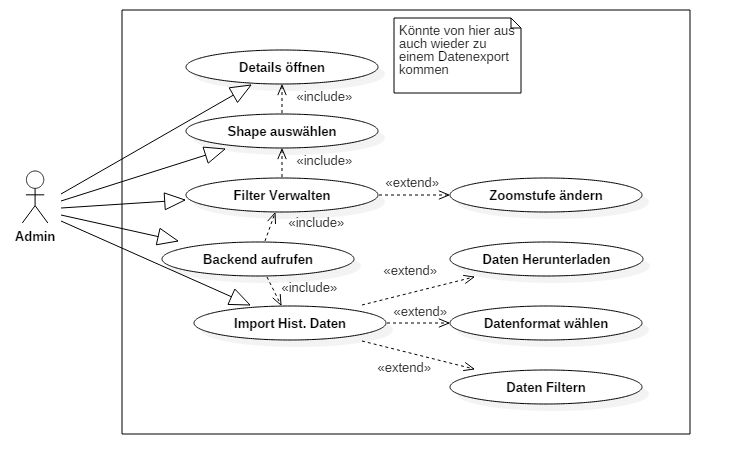
\includegraphics[width=1\linewidth]{diagrams/UseCaseDiagram1.png}
       
       Dieser Anwendungsfall beschreibt die Bedienung des Webinterface. Dem Nutzer stehen folgende Aktionen zur Verfügung:
       \begin{itemize}
            \item Karte anzeigen
            \item Anzeige anpassen
            \item Daten exportieren
            \item Export anpassen
        \end{itemize}
        Nachdem der Nutzer auf das Webinterface zugreift, kann er sich die Karte anzeigen lassen. Diese visualisiert die Daten, welche 
        vom Server durch KafkaStreams bereitgestellt werden. Diese können Echtzeit-, sowie historische Daten enthalten.  Der Server führt 
        im Hintergrund Vorberechnungen zur schnelleren Visualisierung durch. Die Anzeige der Karte, sowie des gesamten Interfaces lässt sich 
        an die Wünsche des Nutzers anpassen, beispielsweise durch die Einbeziehung von Graphen zur besseren Darstellung. Die 
        Datenbestände lassen sich herunterladen und in das gewünschte Format exportieren. Durch Beschränkung der Datenmengen auf 
        bestimmte Zeitintervalle, Datentypen und Wertebereiche kann der Export weiter angepasst werden.
        
    % Anwendungsfall Admin-GUI
    \subsection{Bedienung der Konfigurations-GUI}
        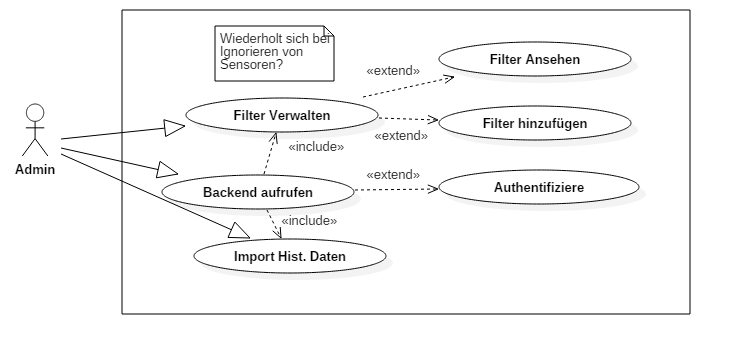
\includegraphics[width=1\linewidth]{diagrams/UseCaseDiagram2.png}
        
        Dieser Anwendungsfall beschreibt die Bedienung der Konfigurations-GUI. Dem Admin stehen folgende Aktionen zur Verfügung:
        \begin{itemize}
            \item Server initialisieren
            \item KafkaStreams verwalten
            \item Datenbestand importieren
            \item Server warten
        \end{itemize}
        Um den Server und damit die Applikation zu starten, greift der Nutzer auf die Konfigurations-GUI zu. Er initialisiert den gestartenen 
        Server, indem ein KafkaStream, bzw. ein Datenbestand eingefügt wird, welcher in einen Stream umgewandelt wird. Dieser wird 
        daraufhin überprüft. Gibt es keine Probleme, so können die Nutzer des Webinterfaces nun die Streams vom Server empfangen. Außerdem ist 
        es nun möglich, die KafkaStreams auf dem Server zu verwalten. Man kann neue Streams hinzufügen, Vorhandene entfernen und 
        enthaltene Sensoren und Sensorendaten anzeigen. Weiterhin lässt sich der Server durch die Konfigurations-GUI warten. Man kann ihn 
        starten, sowie beenden um Analysen durchzuführen und eventuelle Fehler zu beheben.
        
\section{Aktivitätsdiagramm}
    % Aktivitätsdiagramm
    \subsection{}
        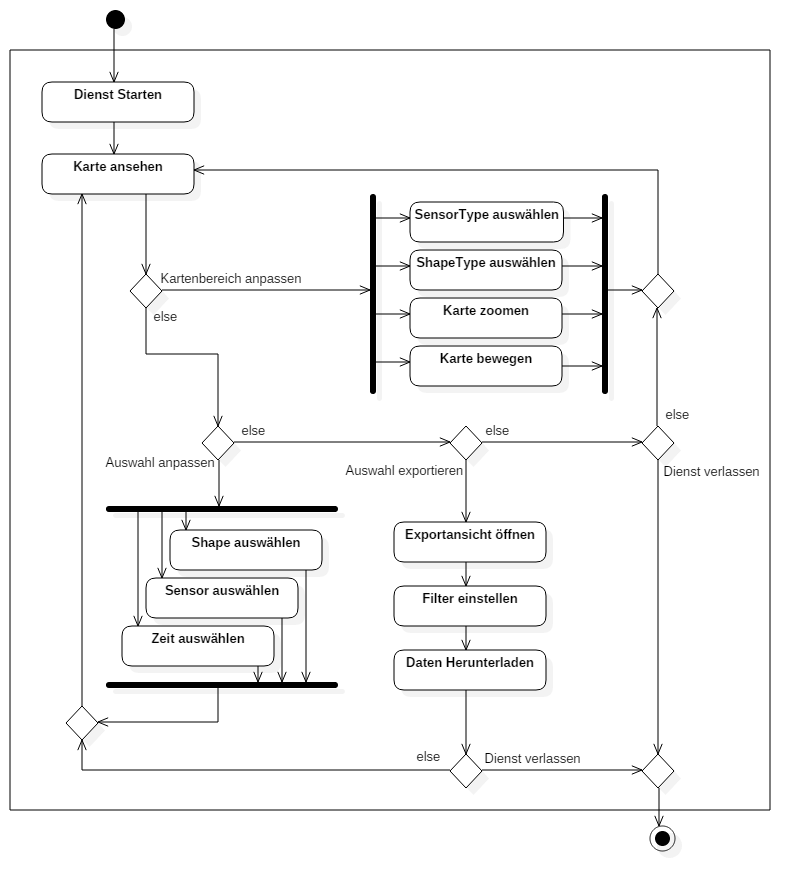
\includegraphics[width=1\linewidth]{diagrams/ActivityDiagram1.png}

        
	\chapter{Benutzeroberfläche}
Die folgenden Darstellungen sollen eine grobe Orientierung für die Benutzeroberflächen des Endprodukts geben. Diese können sich im Verlauf des Projektes noch ändern.
\section{Konfigurations-GUI}
Die Konfigurations-GUI soll einige Optionen bieten, die für reguläre Nutzer des \gls{webinterface} nicht verfügbar sein sollte.

\begin{figure}[H]
	\centering
		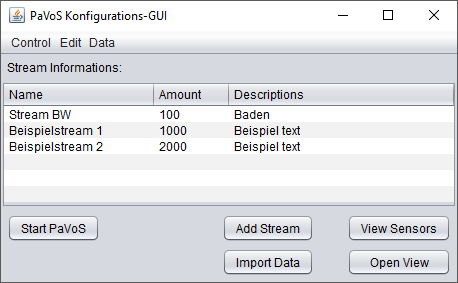
\includegraphics[width=0.6\linewidth]{gui/backend/BackendGUIMain.png}\\
	\caption{Die Konfigurations-GUI zeigt die Streams des Dienstes an. Alle Funktionen sind in den Reitern enthalten. Wichtige Funktionen haben zusätzlich einen Button im unteren Bereich der GUI.}
\end{figure}

\begin{figure}[H]
	\centering
		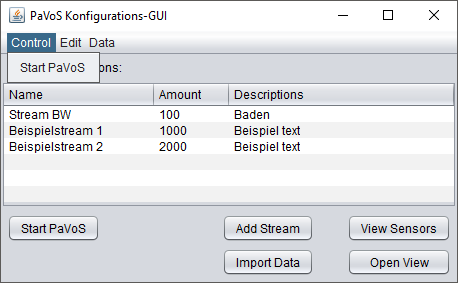
\includegraphics[width=0.6\linewidth]{gui/backend/BackendGUIMenu1.png}\\
	\caption{Control-Reiter: Hier kann der Dienst gestartet und beendet werden.}
\end{figure}

\begin{figure}[H]
	\centering
		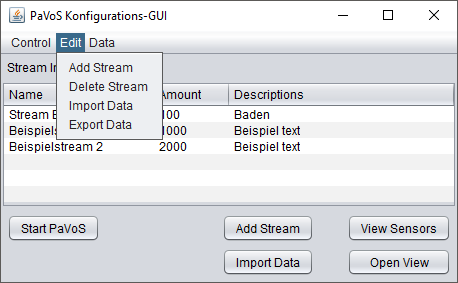
\includegraphics[width=0.6\linewidth]{gui/backend/BackendGUIMenu2.png}\\
	\caption{Edit-Reiter: Dieser Reiter stellt die Funktionen zum hinzufügen oder entfernen der Streams bereit. Außerdem ist es hier möglich Daten zu importieren oder zu exportieren.}
\end{figure}

\begin{figure}[H]
	\centering
		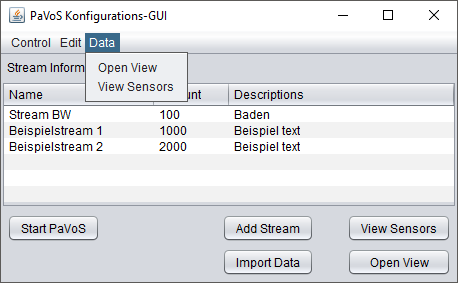
\includegraphics[width=0.6\linewidth]{gui/backend/BackendGUIMenu3.png}\\
	\caption{Data-Reiter: Über den Data-Reiter kann eine Auflistung aller im System enthaltenen \glsdisp{sensor}{Sensoren} angezeigt  oder das Webinterface geöffnet werden.}
\end{figure}
\newpage
\section{Webinterface}
Im Folgenden wird das Webinterface des Dienstes vorgestellt. Diese ist in den Grundzügen vergleichbar mit der von \url{maps.luftdaten.info}, bietet jedoch viele zusätzliche Funktionen an.

\begin{figure}[H]
	\centering
		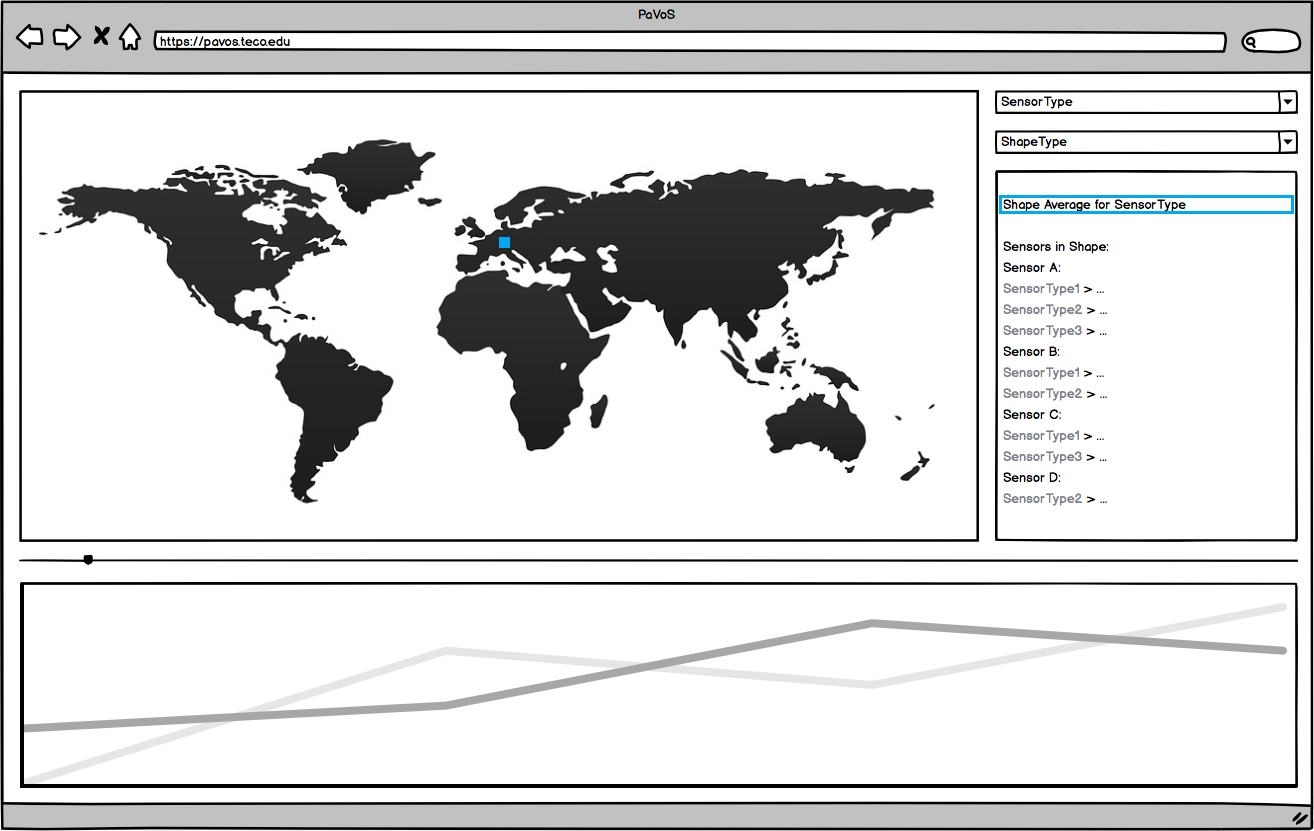
\includegraphics[width=0.9\linewidth]{gui/frontend/FrontGUIWorldWithShapeSelection.png}\\
	\caption{Webinterface mit Weltansicht und ausgewähltem \gls{cluster}.\\
	Dies ist der Startpunkt des Dienstes. Von hier aus können alle angebotenen Features bedient werden. Die Karte besteht aus einer Sammlung von Clustern, die - sofern Sensordaten darin enthalten sind - selektiert werden können, um detaillierte Daten einzusehen.\\
	Hier ist auf der Karte ein Cluster selektiert. In der erweiterten Ansicht wird ``Shape Average for SensorType`` ausgewählt, so werden berechnete Durchschnittsdaten in der Detailansicht angezeigt.}
\end{figure}

\begin{figure}[H]
	\centering
		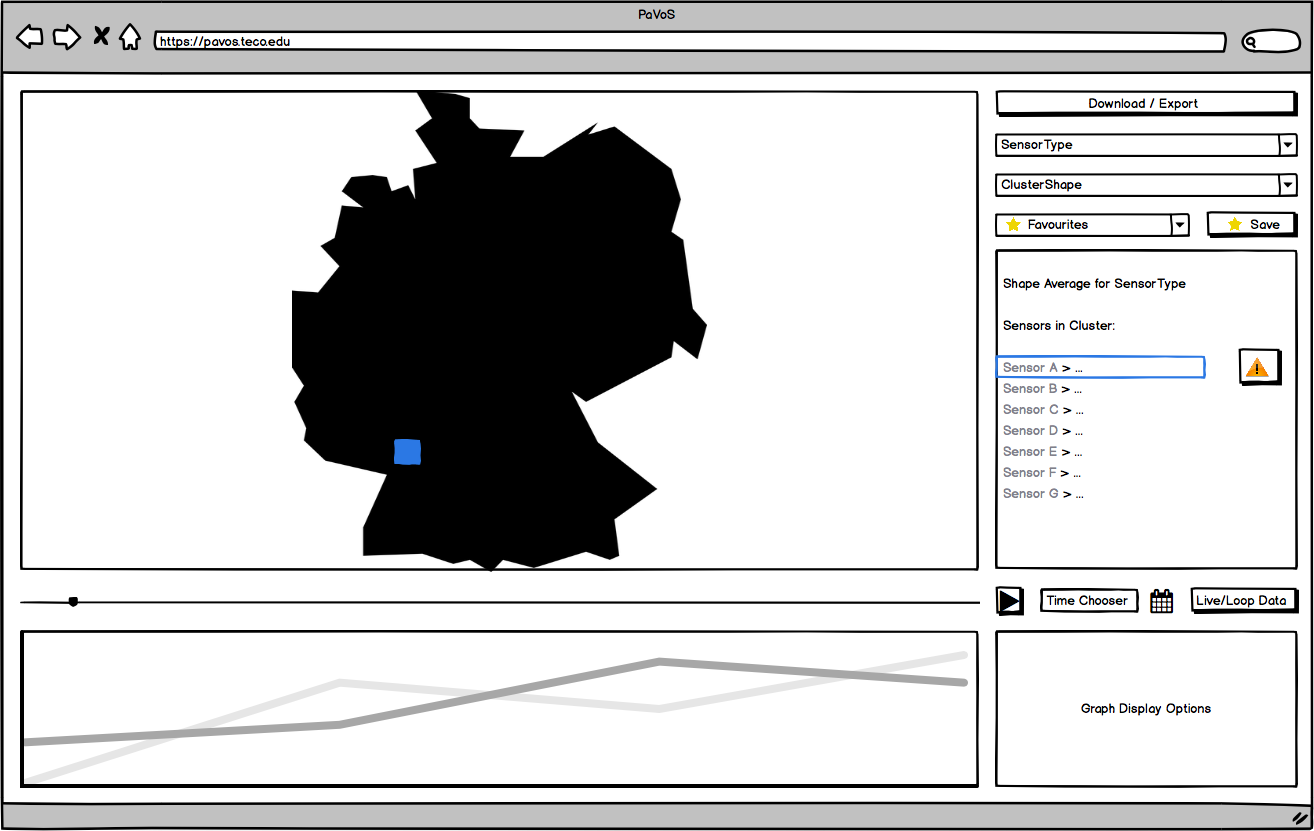
\includegraphics[width=0.9\linewidth]{gui/frontend/FrontGUIGermanyWithShapeSelection.png}\\
	\caption{Webinterface mit Deutschlandansicht und ausgewähltem Cluster.\\
	Hier ist in der erweiterten Ansicht ein bestimmter Sensor selektiert, so werden seine historischen Daten in der Detailansicht angezeigt.}
\end{figure}

\begin{figure}[H]
	\centering
		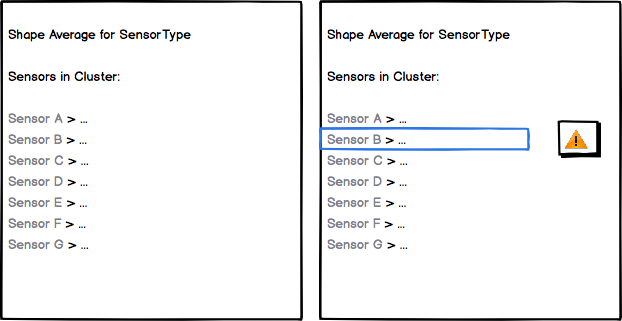
\includegraphics[width=0.8\linewidth]{gui/frontend/FrontGUISensorListAloneAndWithSelection.png}\\
	\caption{Erweiterte Ansicht: Anzeige aller Sensoren innerhalb des ausgewählten Clusters (links). Jeder einzelne Sensor kann ausgewählt werden (rechts), um detaillierte historische Daten anzuzeigen (siehe Detailansicht). Ist ein Sensor ausgewählt, kann er von den Nutzer, unter Angabe eines Grundes, gemeldet werden, indem der Meldebutton genutzt wird (rechts von der Selektion).}
\end{figure}

\begin{figure}[H]
	\centering
	
\includegraphics[width=0.4\linewidth]{gui/frontend/FrontGUISensorType.png}
	\hspace{0.1cm}
	
\includegraphics[width=0.4\linewidth]{gui/frontend/FrontGUIShapeType.png}
	\caption{Dropdown-Listen für den \gls{sensortyp} (SensorType) und die \glsdisp{cluster_shape}{Form des Clusters} (ClusterShape)}
\end{figure}

\begin{figure}[H]
	\centering
	
\includegraphics[width=0.4\linewidth]{gui/frontend/FrontGUIFavourites.png}
	\caption{Dropdown-Liste für die Favoriten und Button zur Speicherung der derzeitigen Selektion als neuer Favorit.}
\end{figure}

\begin{figure}[H]
	\centering
	
\includegraphics[width=0.4\linewidth]{gui/frontend/FrontGUIDownloadButton.png}\\
	\caption{Downloadbutton zum Export von Daten. Wird der Download angefordert, öffnet sich ein Formular, das die genaue Auswahl der gewünschten Daten ermöglicht.}
\end{figure}

\begin{figure}[H]
	\centering
	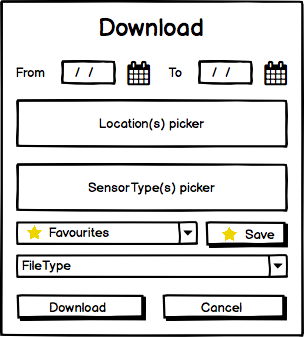
\includegraphics[width=0.5\linewidth]{gui/frontend/FrontGUIExportForm.png}\\
	\caption{Downloadformular zum Export von Daten. Wird der Download angefordert, wird immer zuerst der Download der derzeit ausgewählten Daten angeboten. Das Formular ermöglicht es dem Nutzer den Download nach Zeitintervallen, Lokalitäten und Sensortypen auf seine Bedürfnisse anzupassen. Alternativ können auch gespeicherte Favoriten ausgewählt, oder neue gespeichert werden.}
\end{figure}
\newpage
\begin{figure}[H]
	\centering
	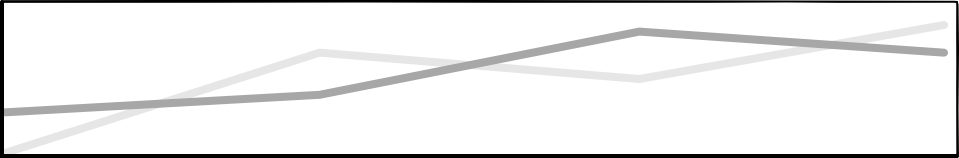
\includegraphics[height=1.5cm]{gui/frontend/FrontGUIDetailGraph.png}
	\hspace{0.1cm}
	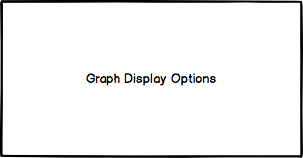
\includegraphics[height=1.5cm]{gui/frontend/FrontGUIGraphSettings.png}
	\caption{Detailansicht: zeitlicher Verlauf spezifischer Sensordaten (Kann ein einzelner Sensor sein, oder der Schnitt eines Clusters). Zusätzlich können rechts Anzeigeoptionen für den Graphen eingestellt werden.}
\end{figure}

\begin{figure}[H]
	\centering
	
\includegraphics[width=0.69\linewidth]{gui/frontend/FrontGUITimeSlider.png}
	\hspace{0.1cm}
	
\includegraphics[width=0.21\linewidth]{gui/frontend/FrontGUITimeSetter.png}
	\caption{Der Zeitregler dient dazu, historische Daten auf der Karte und der erweiterten Ansicht anzuzeigen. Befindet man sich in der Liveansicht, kann man in einen Loop wechseln, der historische Daten in einer Schleife anzeigt. Dieser kann mit dem Play/Pause Button jederzeit unterbrochen oder fortgesetzt werden. Es ist ebenfalls möglich einen gewünschten Zeitpunkt direkt einzugeben. Mit dem Liveansicht-Button kann jederzeit in wieder auf Livedaten gewechselt werden.}
\end{figure}
\newpage
\begin{figure}[H]
	\centering
	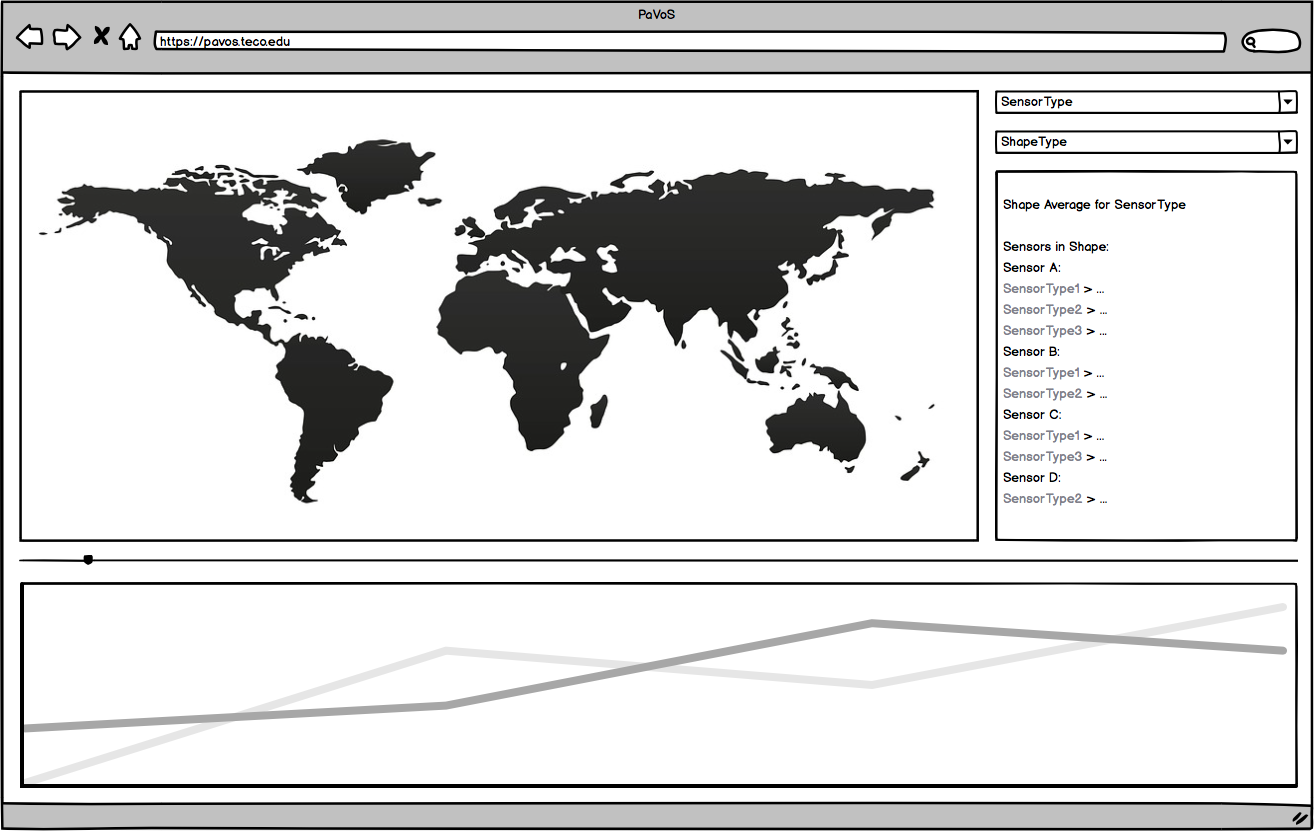
\includegraphics[height=\linewidth, angle=90]{gui/frontend/FrontGUIWorld.png}\\
	\caption{Großansicht Webinterface mit Weltkarte}
\end{figure}
	\chapter{Anhang}
	
	\printglossaries
	\glsaddall
    \newglossaryentry{apache_kafka}{name=Apache Kafka, description={Ein Open-Source-Project der Apache Software Foundation. Dient der Speicherung und Verarbeitung von großen \glsdisp{datenstrom}{Datenströmen}}}
    
    \newglossaryentry{client}{name=Client, description={Nimmt angebotene Dienste des \glsdisp{server}{Servers} wahr}}
    
    \newglossaryentry{cluster}{name=Cluster, description={Eine beliebig große räumliche Ballung und Zusammenfassung von \glsdisp{sensor}{Sensoren} und den dazugehörigen Messwerten}}
    
    \newglossaryentry{cluster_shape}{name=Clustershape, description={Eine geometrische Form, die ein \glsdisp{cluster}{Cluster} und darin enthaltene \glsdisp{sensor}{Sensoren} überdeckt und durch seine Attribute, beispielsweise Färbung und Transparenz, Sensordaten darstellt}}
    
    \newglossaryentry{cookie}{name=Cookie, description={Eine Textinformation, die durch eine Webseite beim Besucher abgelegt wird. Diese kann im weiteren Verlauf von der Seite verarbeitet werden, beispielsweise zum Abrufen von zuvor angegebenen Favoriten}}
    
    \newglossaryentry{csv}{name=CSV, description={Comma-separated values (.csv) ist ein Dateiformat und dient der Speicherung und dem Austausch einfach strukturierter Daten}}
    
    \newglossaryentry{datenstrom}{name=Datenstrom, description={Ein kontinuierlicher Fluss von Datensätzen}}
    
    \newglossaryentry{filter}{name=Filter, description={Eine Beschränkung des Datenbestandes nach vorbestimmten Kriterien}}
    
    \newglossaryentry{frost_server}{name=FROST Server, description={Der Frauenhofer Open Source SensorThings API Server ist eine Implementierung des \glsdisp{ogc}{OGC} Standards und ermöglicht die effiziente Verarbeitung von Sensordaten im \glsdisp{iot}{Internet of Things}}}
    
    \newglossaryentry{iot}{name=Internet of Things, description={Sammelbegriff für die Vernetzung von Gegenständen mit dem und durch das Internet}}
    
    % \newglossaryentry{json}{name=JSON, description={Die JavaScript Object Notation (.json) ist ein kompaktes Datenformat zum Datenauschtausch zwischen Anwendungen}}
    
    \newglossaryentry{master_worker}{name=Master-Worker, description={Master-Worker ist ein hierarchisches Konzept für die Organisation und Verteilung von Aufgaben. Der Master hat dabei volle Kontrolle über die Worker, welche von diesem ihre Aufgaben zugeteilt bekommen}}

    \newglossaryentry{mqtt}{name=MQTT, description={Message Queue Telemetry Transport ist ein offenes Nachrichtenprotokoll für Maschine-zu-Maschine Kommunikation}}
    
    \newglossaryentry{netcdf_glo}{name=NetCDF, description={Das Network Common Data Format (.nc, .cdf) ist ein standardisiertes Dateiformat für den Austausch wissenschaftlicher Daten}}
    
    \newglossaryentry{ogc}{name=OGC, description={Das Open Geospatial Consortium, eine gemeinnützige Organisation die sich auf Standardisierungen bezüglich der computergestützten Verarbeitung insbesondere von Geodaten spezialisiert}}
    
    \newglossaryentry{outlier}{name=Outlier, description={Ein Messwert oder ein Befund, der nicht in eine erwartete Messreihe passt}}
    
    \newglossaryentry{raster}{name=Raster, description={Eine Aufteilung der Karte in \glsdisp{cluster_shape}{Clustershapes} zur besseren Visualisierung}}
    
    % \newglossaryentry{responsive_webdesign}{name=Responsive Webdesign, description={Ein gestalterisches und technisches Paradigma, dass die Erstellung von Webseiten auf Flexibilität auslegt und auf die Merkmale der Endgeräte reagieren lässt}}
   
    \newglossaryentry{sensor}{name=Sensor, description={Ein technisches Bauteil, dass physikalische oder chemische Eigenschaften seiner Umgebung qualitativ oder quantitativ erfassen kann}}
    
    % Oder lieber Datentyp ?
    \newglossaryentry{sensordatentyp}{name=Sensordatentyp, description={Die Art des Messwerts, der durch einen \glsdisp{sensor}{Sensor} erfasst wird, beispielsweise Feinstaub, Temperatur, Luftfeuchtigkeit oder Windstärke}}
    
    \newglossaryentry{server}{name=Server, description={Ein Computer/Computerprogramm, dass Dienstprogramme, Daten oder andere Ressourcen für \glsdisp{client}{Clients} bereitstellt}}
    
    % \newglossaryentry{split_panel}{name=Split Panel, description={Die Darstellung zweier oder mehr Datensätze nebeneinander zum besseren Vergleich}}
    
    \newglossaryentry{webinterface}{name=Webinterface, description={Eine Programmschnittstelle, die über einen Internetbrowser angesprochen werden kann}}

\end{document}